\paragraph{}
in this section we will mention our final model and its performance.
we Have Three combinations we will illustrate.

\begin{enumerate}
	\item CNN see figure. \ref{cnn}
	\item Hog and Landmarks see figure. \ref{lm+hog}
	\item CNN with Hog and Landmarks see figure. \ref{cnn_lm_hog}
\end{enumerate}

\begin{figure}
	\centering
	\label{cnn}
	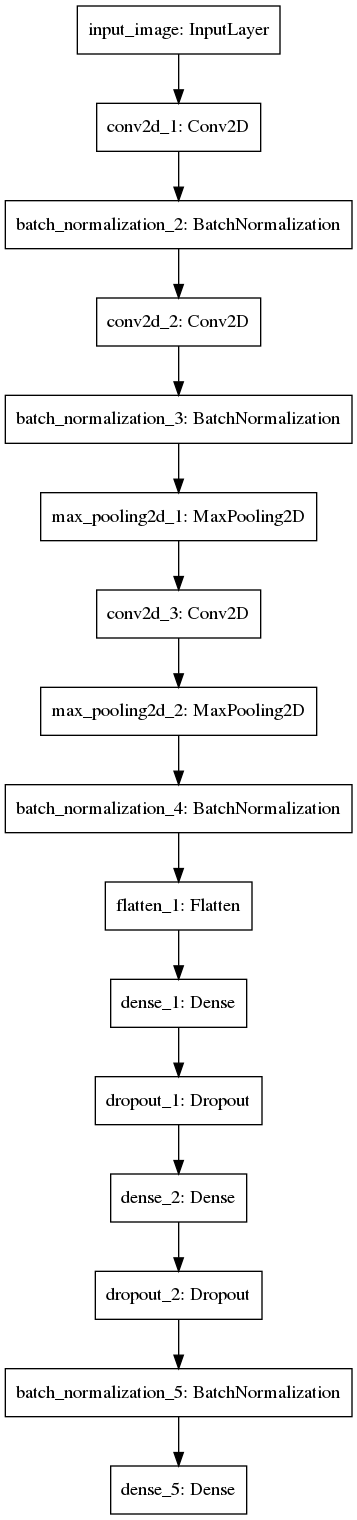
\includegraphics[width=.3\textwidth]{images/cnn.png}
	\caption{Diagram of CNN structure}
\end{figure}

\begin{figure}
	\centering
	\label{lm+hog}
	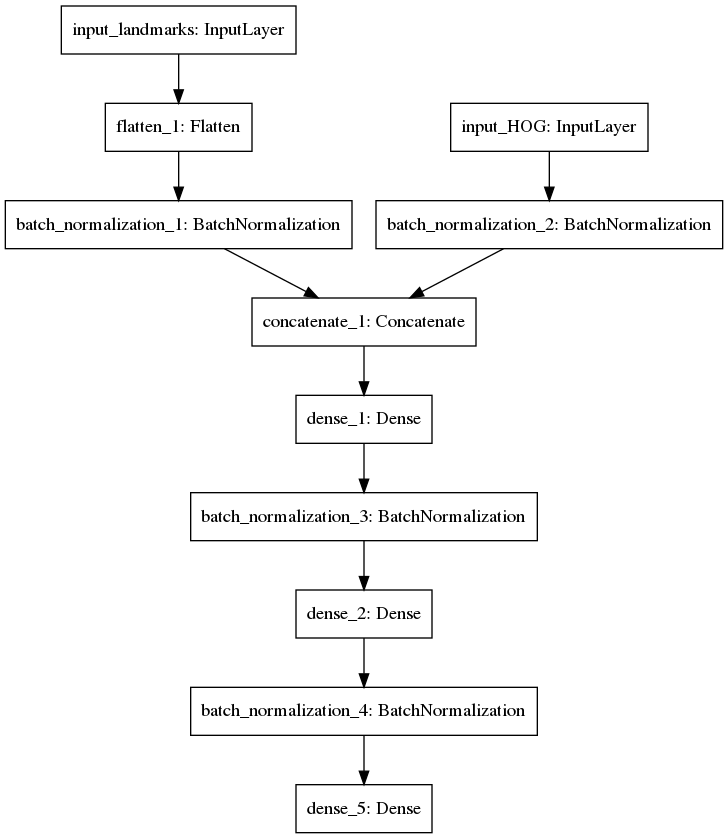
\includegraphics[width=.8\textwidth]{images/hog_lm.png}
	\caption{Diagram of hog and landmarks structure}
\end{figure}
\begin{figure}
	\centering
	\label{cnn_lm_hog}
	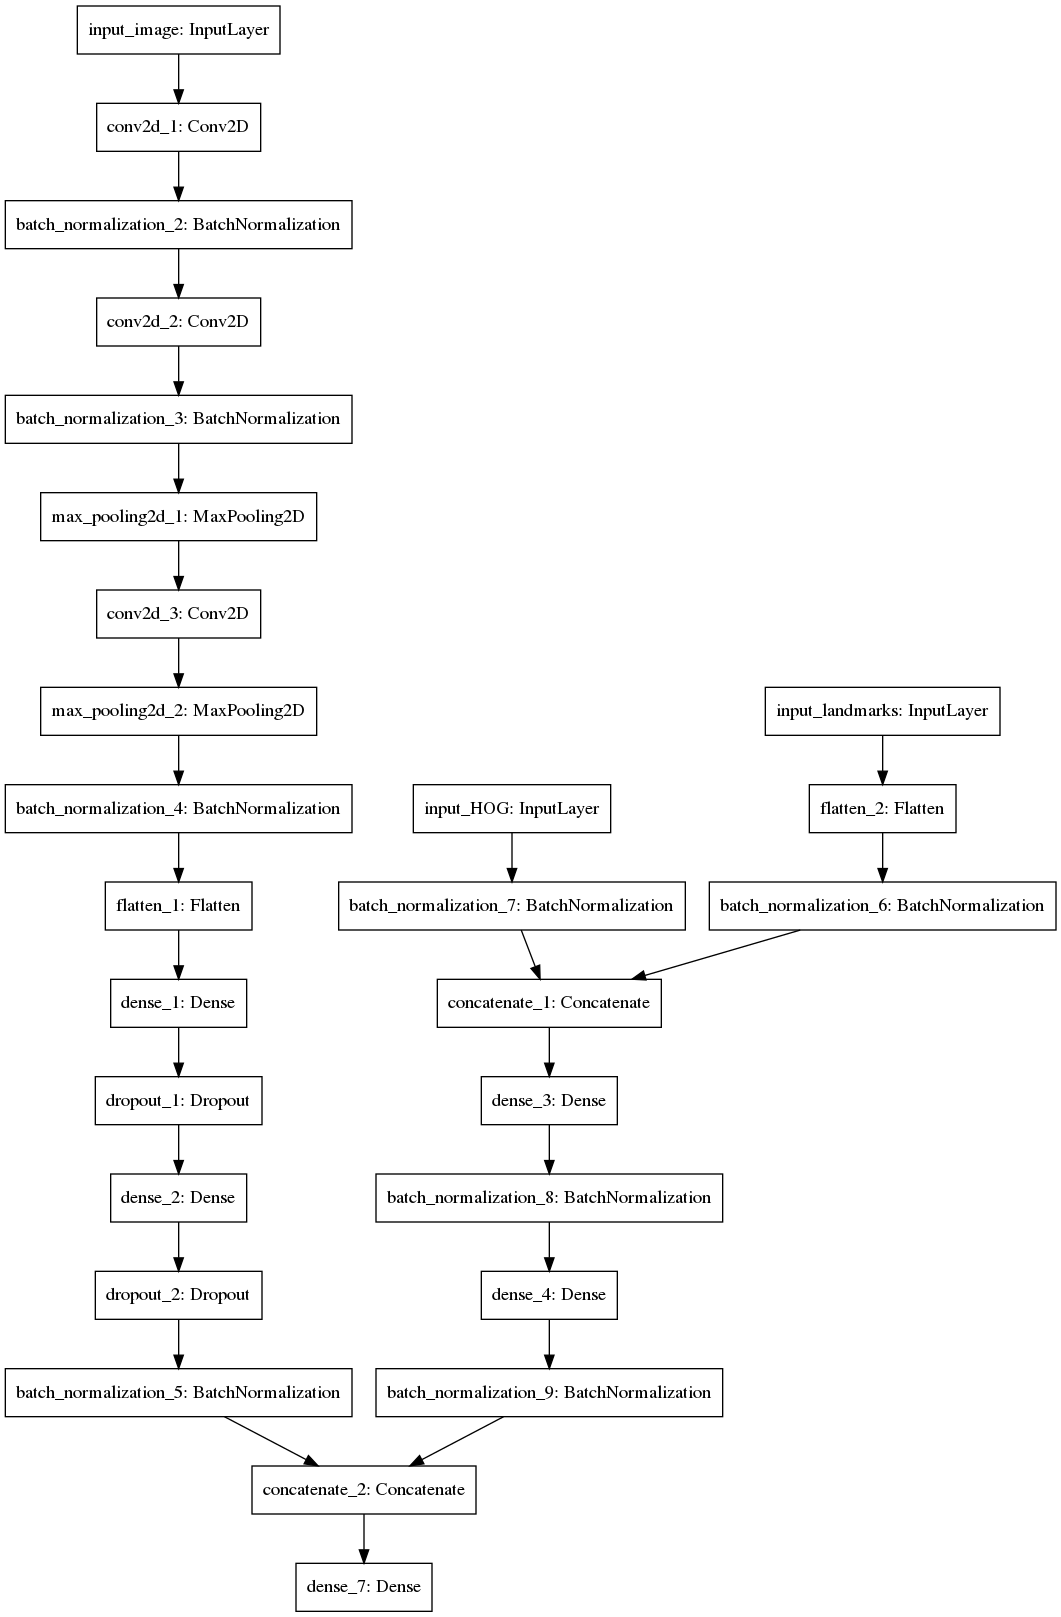
\includegraphics[width=.8\textwidth]{images/cnn_hog_lm.png}
	\caption{Diagram of cnn+hog+lm structure}
\end{figure}
\paragraph{}
We finally choose the model with only landmarks and hog path with final accuracy 98\% on the combination of ck+ and RafD dataset as the working model as we notice that :
\begin{enumerate}
	\item Using landmarks and hog as a feature extraction then feed it to model layers as described in the figure \ref{lm+hog} give a good accuracy with small model size (1M) and the Training Process itself is too fast comparing with Cnn
	\item Using cnn model only \ref{cnn} work good give the same accuracy but the model size is large and take to much time in training .
	\item combine cnn with landmarks and hog as in \ref{cnn_lm_hog} it does not make any sense as cnn itself make its feature extraction so but it with hog and landmarks make no difference in the accuracy only make model size bigger and make training process harder. 
\end{enumerate} 